

\title{Efficient Real-Time Fire Surveillance: A Lightweight
Motion-Heuristic Skip Module for Accelerated Inference}
\author{Hoang Van-Ha, Jong Weon Lee, Park Chun-Su}
\date{2026.04.10}

\begin{document}
\maketitle
\begin{abstract}
Conventional deep learning (DL)-based fire and smoke detection systems
process every frame of a video stream through a computationally
intensive model to classify the presence of fire or smoke. However, in
surveillance scenarios --- particularly indoor environments --- video
streams frequently contain static, background-only frames devoid of
motion or relevant events, rendering per-frame inference redundant and
wasteful of computational resources. To address this limitation, this
study proposes a novel skip-module mechanism that leverages motion
detection to selectively bypass DL inference on non-informative frames
in fire and smoke classification pipelines. Evaluation on a large-scale
dataset comprising 150 indoor videos demonstrates that the proposed
method substantially improves processing throughput while preserving
detection performance. Specifically, the skip module enable the system a
30\% increase in frames per second (FPS) with a minimal reduction in
recall of only 1\% relative to the baseline (recall ≥ 95\%),
demonstrating the feasibility of plug-and-play inference acceleration
for real-time fire and smoke surveillance systems.
\end{abstract}

\section{Introduction}\label{sec:introduction}

Fires and wildfires, if not detected and controlled in their early
stages, can quickly escalate --- especially under dry and windy
conditions --- resulting in catastrophic consequences including loss of
life, destruction of property, and damage to natural ecosystems. For
instance, in 2017, urban fires and wildfires in California, USA, caused
an estimated economic loss of 10 billion USD
\citeproc{ref-californiafire:online}{{[}1{]}}. More recently, in 2025, a
forest fire in Gyeongsang Province, South Korea, burned approximately
90,000 acres, resulting in at least 27 fatalities and the evacuation of
nearly 40,000 residents \citeproc{ref-southkoreafire:online}{{[}2{]}}.
Automated early-stage fire and smoke detection systems are therefore
critical for enabling timely intervention and minimizing damage.

Numerous fire and smoke detection methods leveraging deep learning (DL)
have been proposed in recent years
\citeproc{ref-cheng2024visual}{{[}3{]}},
\citeproc{ref-gragnaniello2024fire}{{[}4{]}}. In practical deployments,
these systems are commonly applied to CCTV video streams, where DL-based
classifiers or object detectors perform inference on each frame
individually. Although this frame-wise paradigm is straightforward to
implement, it exhibits two key limitations. First, it relies exclusively
on spatial information within individual frames, neglecting temporal
cues --- such as motion --- inherent in video data. Second, in
surveillance scenarios, particularly in indoor environments, consecutive
frames often exhibit minimal variation due to static scene content.
Applying a DL model indiscriminately to every frame under such
conditions is computationally redundant, increasing processing cost and
latency without contributing to detection performance. This inefficiency
is further compounded by the well-known accuracy--efficiency trade-off
in DL: more accurate models are generally more computationally
intensive, and redundant frame processing amplifies these demands,
rendering real-time performance difficult to achieve.

A common strategy to reduce inference cost is to substitute a heavy,
high-accuracy DL model with a lighter alternative; however, this
typically degrades detection reliability --- an unacceptable compromise
in safety-critical applications such as fire and smoke detection. This
study takes a complementary approach: rather than replacing the
classifier, we introduce a lightweight skip-module that acts as a
computational gate, selectively forwarding only frames with significant
scene activity to the high-capacity classifier while bypassing static,
non-informative frames. As illustrated in Fig. \ref{fig:pipeline}, the
conventional pipeline processes every frame through the classifier,
whereas the proposed pipeline inserts the skip-module upstream to
conditionally suppress redundant inference calls.

In particular, our main contributions are summarized as follows:

\begin{itemize}
\item
  \textbf{Skip-Module Mechanism:} We propose a lightweight skip-module
  that exploits motion estimation via frame differencing to identify
  static scenes and bypass DL inference on non-informative frames,
  reducing computational cost without modifying the underlying
  classifier. The module is designed as a plug-and-play component
  compatible with existing fire and smoke detection pipelines. To
  identify the optimal operating configuration, we further develop a
  systematic hyperparameter optimization procedure that maximizes
  throughput while preserving detection performance.
\item
  \textbf{Indoor Fire and Smoke Video Dataset:} We construct an
  annotated dataset comprising 150 indoor fire and smoke videos ---
  including fire, smoke, and background-only classes --- captured by
  static surveillance cameras at resolutions from 720p to 1080p. The
  dataset covers diverse environments such as warehouses, parking areas,
  and offices under varying lighting conditions, providing a realistic
  benchmark for evaluating detection systems in static surveillance
  scenarios.
\item
  \textbf{Comprehensive System Evaluation:} We integrate the skip-module
  with a high-capacity DL classifier (BIG model) and evaluate the
  combined system on our video dataset against the baseline (BIG model
  without skipping) and existing methods. Results demonstrate a 30\%
  improvement in FPS with a recall reduction of less than 1\%, alongside
  an ablation study that provides insights into system performance and
  limitations.
\end{itemize}

The rest of this paper is organized as follows:
Section~\ref{sec:relatedWork} reviews existing fire and smoke detection
methods for video and relevant motion detection techniques,
contextualizing the need for efficient processing in static surveillance
scenarios. Section~\ref{sec:method} describes the proposed system
architecture, the design of the skip-module, its integration with the
BIG model, and the hyperparameter optimization strategy.
Section~\ref{sec:results} presents the experimental setup, evaluation
metrics, and performance results on our large-scale indoor video
dataset. Finally, Section~\ref{sec:conclusion} summarizes the key
findings and discusses limitations and future research directions.



\section{The proposed method}\label{sec:method}

\subsection{System Overview}\label{system-overview}

\begin{figure}[ht]
  \centering
  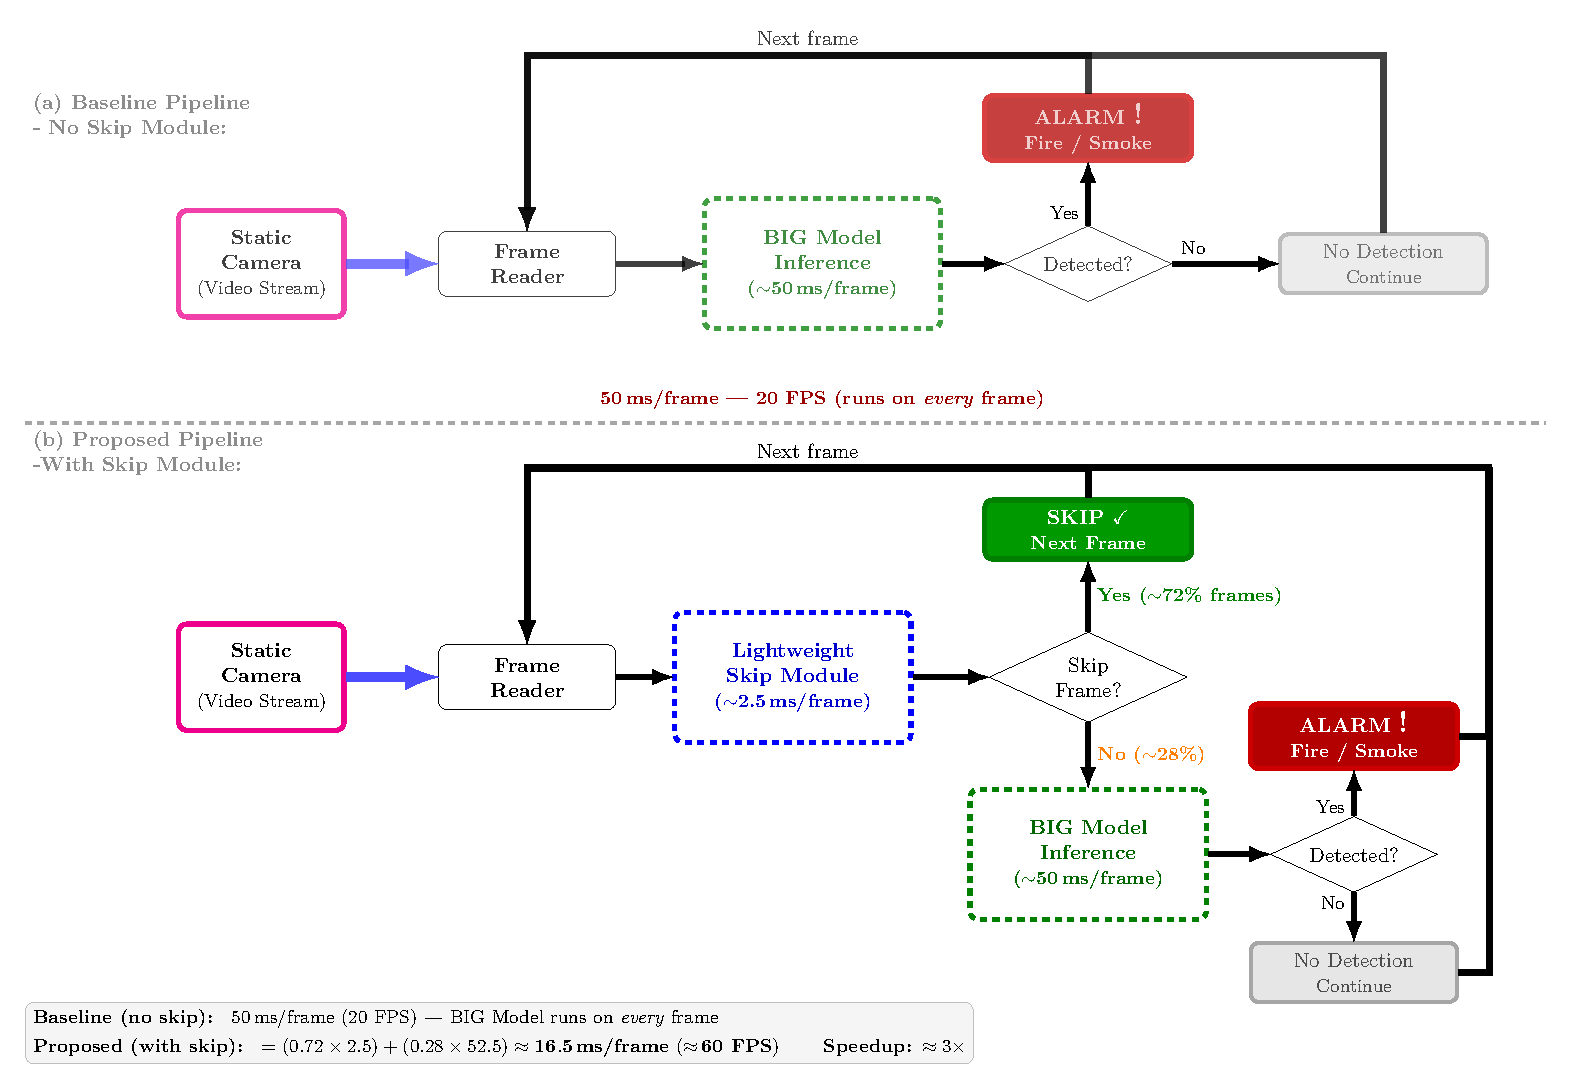
\includegraphics[width=\linewidth,keepaspectratio, scale=0.3]{3.fig/fig_pipeline.pdf}
  \caption{Proposed pipeline with Skip Frame Mechanism for Indoor Fire and Smoke Detection}\label{fig:pipeline}
\end{figure}

The proposed system is a fire and smoke detection pipeline that
processes a continuous video stream and classifies each frame as either
containing fire/smoke or not. The core idea is to extend the
conventional pipeline with a lightweight \textbf{skip module}
\(\mathcal{S}\), which acts as a gating mechanism to suppress
unnecessary inferences on non-informative frames, thereby improving
computational efficiency. Formally, let \(f_t\) denote the video frame
at time step \(t\), \(\mathcal{M}\) the DL classifier, and
\(\hat{y}_t \in \{0, 1\}\) the predicted label for \(f_t\).

\textbf{Baseline system.} Each frame is directly passed to the
classifier:

\[\hat{y}_t = \mathcal{M}(f_t)\]

\textbf{Proposed system.} The skip module \(\mathcal{S}\) first
evaluates \(f_t\) using inter-frame motion cues or other information and
outputs a binary gate decision \(s_t\). The full system output becomes:

\[\hat{y}_t = \begin{cases} \mathcal{M}(f_t) & \text{if } s_t = 1 \quad
\text{(run inference)} \\ 0 & \text{if } s_t = 0 \quad \text{(skip, label as
negative)} \end{cases}\]

In this work, \(\mathcal{S}\) derives \(s_t\) from the motion estimated
between \(f_t\) and the previous frame \(f_{t-1}\). Frames with little
or no motion are unlikely to contain fire or smoke, and are therefore
skipped without invoking \(\mathcal{M}\). The model \(\mathcal{M}\) is
typically a high-capacity, accurate classifier but is computationally
expensive. The skip module \(\mathcal{S}\) is intentionally lightweight,
adding negligible overhead. The goal of \(\mathcal{S}\) is to skip as
many true-negative frames as possible while minimizing the risk of
skipping true-positive frames, thus improving overall system throughput
(FPS) while maintaining high accuracy for fire/smoke detection.

\subsection{Skip Module Design}\label{skip-module-design}

\begin{figure}[htbp]
  \centering
  
\includegraphics[width=\linewidth,keepaspectratio, scale=0.3]{3.fig/fig_skip_module.pdf}
  \caption{Skip Module for Fire and Smoke Detection}\label{fig:skipmodule}
\end{figure}

\begin{algorithm}[ht]
	\caption{Skip Module $\mathcal{S}$: Motion-Based Frame Gating}
	\label{alg:skipmodule}
	\begin{algorithmic}[1]

		\Require Video stream $\{f_1, f_2, \dots\}$, motion detector $\mathcal{D}$,
		scale factor $\alpha$, block size $B$, block active threshold $\tau$
		\Ensure Skip decisions $\{s_1, s_2, \dots\}$, where $s_t \in \{0,1\}$

		\State $f_{\text{prev}} \leftarrow \text{null}$ \Comment{Initialize previous frame}

		\For{each incoming frame $f_t$}

		\Statex \hspace{1.5em} \textbf{Step 1: Pre-process}
		\State Downsample $f_t$ by $\alpha$ to obtain $\tilde{f}_t$
		\State Let $B_s \leftarrow B \cdot \alpha$ \Comment{Effective block size on downsampled frame}
		\State Pad $\tilde{f}_t$ to be divisible by $B_s$

		\Statex \hspace{1.5em} \textbf{Step 2: Compute Foreground Mask}
		\If{$f_{\text{prev}} = \text{null}$} \Comment{No previous frame on first iteration}
		\State $s_t \leftarrow 1$ \Comment{Run inference on first frame}
		\State $f_{\text{prev}} \leftarrow \tilde{f}_t$
		\State \textbf{continue}
		\EndIf
		\State $\mathbf{M}_t \leftarrow \mathcal{D}(\tilde{f}_t,\, f_{\text{prev}})$ \Comment{$\mathcal{D}$: e.g., FrameDiff or AccMotionDet}
		\State Partition $\mathbf{M}_t$ into a grid of non-overlapping blocks of size $B_s$
		\State Mark a block as \textit{active} if its foreground pixel ratio $> \tau$

		\Statex \hspace{1.5em} \textbf{Step 3: Gating Decision}
		\If{any active block exists}
		\State $s_t \leftarrow 1$ \Comment{Motion detected, run DL inference}
		\Else
		\State $s_t \leftarrow 0$ \Comment{No motion, skip inference}
		\EndIf

		\State $f_{\text{prev}} \leftarrow \tilde{f}_t$ \Comment{Update previous frame for next iteration}
		\State \textbf{yield} $s_t$

		\EndFor

	\end{algorithmic}
\end{algorithm}

As noted above, \(\mathcal{S}\) can leverage any available information
--- such as motion, color, or texture --- to compute the skip decision
\(s_t\). In this work, we focus on motion information derived from
consecutive frames as the primary cue. Specifically, we design and
evaluate two motion-based instantiations of \(\mathcal{S}\): (1) a frame
differencing method, and (2) a motion accumulation method. Both
approaches are selected for their simplicity and low computational cost,
making them well-suited for real-time deployment. The overall workflow
of \(\mathcal{S}\) is illustrated in Figure \ref{fig:skipmodule} and the
detailed algorithms are described in the Algorithm \ref{alg:skipmodule}.

\subsubsection{FrameDiffDet --- Naive Motion
Detection}\label{framediffdet-naive-motion-detection}

\noindent
Let $F_t$ denote the grayscale frame at time $t$, converted from the
downsampled input $\tilde{f}_t$.
$\mathbf{M}_t \in \{0, 255\}$ is the binary foreground mask output,
where a pixel is declared active if the absolute inter-frame intensity
change exceeds threshold $\tau_d$. The algorithm is formalized in Algorithm~\ref{alg:framediff_det}.

\begin{algorithm}[ht]
\caption{Frame Difference Detector (FrameDiffDet)}
\label{alg:framediff_det}
\begin{algorithmic}[1]

\Require Downsampled frames $\tilde{f}_t,\, f_{\text{prev}}$
\Require $\tau_d$: pixel difference sensitivity threshold
\Ensure $\mathbf{M}_t \in \{0, 255\}$: binary foreground mask

\Statex

\State Convert $\tilde{f}_t$ and $f_{\text{prev}}$ to grayscale: $F_t,\, F_{\text{prev}}$

\Statex

\State $\mathbf{M}_t(i,j) \leftarrow
\begin{cases}
255 & |F_t(i,j) - F_{\text{prev}}(i,j)| > \tau_d \\
0   & \text{otherwise}
\end{cases}$

\State \Return $\mathbf{M}_t$

\end{algorithmic}
\end{algorithm}

\subsubsection{AccMotionDet --- Motion Detection with
Accumulation}\label{accmotiondet-motion-detection-with-accumulation}

\noindent
The details of the AccMotionDet algorithm are outlined in
Algorithm~\ref{alg:acc_motion_det}. Let $F_t$ denote the grayscale frame at time
$t$, converted from the
downsampled input $\tilde{f}_t$, and $\mathbf{K}_t \in [0, K_{\max}]$
the per-pixel \textit{accumulated motion mask}.
Upon detection, $\mathbf{K}_t$ is incremented by $\omega$ and decays
by $\delta$ each frame, bounded at $K_{\max}$ to prevent indefinite
accumulation of stale evidence.
A pixel is declared active only when $\mathbf{K}_t \geq \tau_m$,
suppressing transient noise and single-frame flicker.
The binary output $\mathbf{M}_t \in \{0, 255\}$ is consistent with
the interface expected by the skip module $\mathcal{S}$.

\begin{algorithm}[ht]
\caption{Accumulation Motion Detector (AccMotionDet)}
\label{alg:acc_motion_det}
\begin{algorithmic}[1]

\Require Downsampled frames $\tilde{f}_t,\, f_{\text{prev}}$;
         accumulated mask $\mathbf{K}_{t-1}$ (initialized to $\mathbf{0}$)
\Require $\tau_d$: pixel difference sensitivity,\;
         $\omega$: motion increment,\;
         $\tau_m$: activation threshold,\;
         $K_{\max}$: accumulation cap,\;
         $\delta$: decay rate
\Ensure $\mathbf{M}_t \in \{0, 255\}$: binary foreground mask;\;
        $\mathbf{K}_t$: updated accumulated mask

\Statex

\State Convert $\tilde{f}_t$ and $f_{\text{prev}}$ to grayscale: $F_t,\, F_{\text{prev}}$

\Statex

\State $\mathbf{D}_t \leftarrow \left| F_t - F_{\text{prev}} \right|$
\Comment{Absolute inter-frame difference}

\State $\symbf{\Delta}_t(i,j) \leftarrow
\begin{cases}
\omega & \mathbf{D}_t(i,j) > \tau_d \\
0      & \text{otherwise}
\end{cases}$
\Comment{Instantaneous increment map}

\Statex

\State $\mathbf{K}_t \leftarrow \min\!\left(\mathbf{K}_{t-1} + \symbf{\Delta}_t,\; K_{\max}\right)$
\Comment{Accumulate and cap}

\State $\mathbf{K}_t \leftarrow \max\!\left(\mathbf{K}_t - \delta,\; 0\right)$
\Comment{Temporal decay}

\Statex

\State $\mathbf{M}_t(i,j) \leftarrow
\begin{cases}
255 & \mathbf{K}_t(i,j) \geq \tau_m \\
0   & \text{otherwise}
\end{cases}$
\Comment{Threshold to binary mask}

\State \Return $\mathbf{M}_t,\; \mathbf{K}_t$

\end{algorithmic}
\end{algorithm}

\subsection{Skip Module Hyperparameter
Optimization}\label{sec:hyperparam}

\begin{algorithm}[htbp]
\caption{Skip Module Hyperparameter Selection}
\label{alg:hyperparam}
\begin{algorithmic}[1]

\Require Parameter space $\Theta$, validation set $D_{\text{val}}$,
DL model $\mathcal{M}$, recall tolerance $\delta_R$,
overhead ratio $\beta$, weights $w_S, w_R$
\Ensure Optimal parameters $\theta^*$

\State baseline $\gets$ \textsc{EvaluatePipeline}($D_{\text{val}}$, skip=None, $\mathcal{M}$)
\State Extract $R_{\text{base}}$, $T_{\text{DL}}$ from baseline
\State best\_score $\gets -\infty$; \quad $\theta^* \gets$ None

\For{each $\theta \in \Theta$}
\State results $\gets$ \textsc{EvaluatePipeline}($D_{\text{val}}$, $\mathcal{S}(\theta)$, $\mathcal{M}$)
\State Extract $R(\theta)$, $S_r(\theta)$, $T_{\text{skip}}(\theta)$ from results
\If{$R(\theta) \geq R_{\text{base}} - \delta_R$
\textbf{ and }
$T_{\text{skip}}(\theta) \leq \beta \cdot T_{\text{DL}}$}
\State $\rho(\theta) \gets 1 - \dfrac{R_{\text{base}} - R(\theta)}{\delta_R}$
\State score $\gets w_S\, S_r(\theta) + w_R\, \rho(\theta)$
\If{score $>$ best\_score}
\State best\_score $\gets$ score
\State $\theta^* \gets \theta$
\EndIf
\EndIf
\EndFor

\State \Return $\theta^*$

\end{algorithmic}
\end{algorithm}

The skip module $\mathcal{S}$ contains several hyperparameters (e.g., motion
threshold, accumulation window size) that can significantly impact the
performance of the overall system. To identify the optimal configuration, we
employ a grid search based hyperparameter optimization procedure on a validation
set $D_{\text{val}}$ derived from our video dataset with respect to several
system-wide metrics defined in Section~\ref{sec:metrics}. More specifically, to
select the optimal hyperparameters for the proposed skip module, we employ a
constrained optimization procedure on the validation set $D_{\text{val}}$. Let
$R_{\text{base}}$ denote the baseline recall, i.e., the fraction of fire/smoke
frames correctly detected by the pipeline without skipping, and let $T_{\text{DL}}$
denote its mean per-frame inference time. For each candidate parameter set
$\theta \in \Theta$ obtained by grid search, we evaluate the full pipeline
$\text{Read} \rightarrow \mathcal{S}(\theta) \rightarrow [\mathcal{M}]$ and
compute three metrics: recall $R(\theta)$ (the fraction of fire/smoke frames
correctly detected), skip rate $S_r(\theta)$ (the fraction of ground-truth
negative frames skipped by $\mathcal{S}$), and mean per-frame skip module time
$T_{\text{skip}}(\theta)$. Formal metric definitions are given in
Section~\ref{sec:metrics}.

The skip rate $S_r(\theta)$ is computed on $D_{\text{val}}$ following the
definition in Section~\ref{sec:metrics}, with $N_{\text{neg}}$ instantiated as
$N_{\text{neg}}^{\text{val}} = |\{f_i \in D_{\text{val}} : y_i = 0\}|$, which
is fixed by the validation set and independent of $\theta$.

The mean per-frame inference times are defined as:
\begin{equation}
    T_{\text{DL}} = \frac{1}{|D_{\text{val}}|}
    \sum_{i=1}^{|D_{\text{val}}|} t_{\text{DL}}(f_i),
\end{equation}
\begin{equation}
    T_{\text{skip}}(\theta) = \frac{1}{|D_{\text{val}}|}
    \sum_{i=1}^{|D_{\text{val}}|} t_{\text{skip}}(f_i, \theta),
\end{equation}
where $f_i$ denotes the $i$-th frame in $D_{\text{val}}$, and both averages are
taken over all frames to reflect the runtime cost on a typical video stream.

\textbf{Feasibility constraints.} A candidate $\theta$ is considered feasible
only if it satisfies two hard constraints:
\begin{equation}
    R(\theta) \geq R_{\text{base}} - \delta_R,
\end{equation}
\begin{equation}
    T_{\text{skip}}(\theta) \leq \beta \cdot T_{\text{DL}},
\end{equation}
where recall tolerance $\delta_R > 0$ is the maximum allowable absolute recall
drop, and overhead ratio $\beta \in (0, 1)$ bounds the skip module overhead as
a fraction of one full DL inference. For example, setting $\delta_R = 0.01$ and
$\beta = 0.10$ means the system tolerates at most a 1\% recall drop and requires
the skip module to run within 10\% of the cost of a single DL inference.

\textbf{Scoring feasible candidates.} Among feasible candidates, the only term
that requires explicit optimization is recall retention, defined as
\begin{equation}
    \rho(\theta) = 1 - \frac{R_{\text{base}} - R(\theta)}{\delta_R},
\end{equation}
which equals $1$ when recall matches the baseline and $0$ when recall reaches
the lowest acceptable level $R_{\text{base}} - \delta_R$. This term is bounded
in $[0, 1]$ over the feasible region, making it directly comparable to
$S_r(\theta)$ in the weighted score.

\textbf{Optimal selection.} The optimal parameter set $\theta^*$ is selected as
\begin{equation}
    \theta^* = \arg\max_{\theta \in \Theta_{\text{feasible}}}
    \left[ w_R\,\rho(\theta) + w_S\,S_r(\theta) \right],
\end{equation}
where $\Theta_{\text{feasible}} = \{\theta \in \Theta : R(\theta) \geq
R_{\text{base}} - \delta_R \text{ and } T_{\text{skip}}(\theta) \leq \beta
\cdot T_{\text{DL}}\}$, and the nonnegative weights satisfy $w_S + w_R = 1$.

\textbf{FAR of the skip-enabled system.} The skip module $\mathcal{S}$ acts as
a conservative gate: skipped frames are labeled negative directly, while passed
frames are processed by the same downstream detector $\mathcal{M}$ as in the
baseline. Therefore, every false alarm produced by the skip-enabled system is
also present in the baseline, implying
\begin{equation}
    \mathrm{FAR}(\theta) \leq \mathrm{FAR}_{\text{base}},
\end{equation}
where $\mathrm{FAR}(\theta)$ and $\mathrm{FAR}_{\text{base}}$ denote the false
alarm rates of the skip-enabled and baseline systems, respectively. The primary
safety risk is recall degradation caused by incorrectly skipped fire/smoke
frames, which motivates enforcing the recall constraint as a hard gate prior to
any candidate ranking.

% !=======================================================
% ! Start justification here 0
\textbf{Why excluding FAR-based terms from the scoring objective.}
We show that, under a mild independence assumption, the expected false
alarm rate ($\mathrm{FAR}(\theta)$) of the skip-enabled system is
entirely determined by the skip rate $S_r(\theta)$ and the fixed
baseline constant $\mathrm{FAR}_{\text{base}}$. This implies that any
scoring term depending on the expected FAR is redundant with $S_r(\theta)$
and adds no independent optimization signal.

By definition, the FAR of the skip-enabled system is:
\begin{equation}
    \mathrm{FAR}(\theta) = \frac{FP(\theta)}{N_{\text{neg}}}
\end{equation}
where $N_{\text{neg}}$ is the total number of ground-truth negative
frames, and $FP(\theta)$ is the number of false positives produced.

Since every skipped frame is assigned a negative label ($0$), it cannot
trigger a false positive. Therefore, the total number of false positives
is exactly the baseline false positives minus the baseline false
positives that were skipped:
\begin{equation}
    FP(\theta) = FP_{\text{base}} - a
\end{equation}
where $FP_{\text{base}}$ is the baseline false positive count, and $a$
is the number of skipped frames that the baseline model would have
misclassified. Taking the expectation yields:
\begin{equation}
    \mathbb{E}[\mathrm{FAR}(\theta)]
    = \frac{FP_{\text{base}} - \mathbb{E}[a]}{N_{\text{neg}}}
\end{equation}

The skip module $\mathcal{S}$ operates solely on inter-frame motion,
independent of the baseline model $\mathcal{M}$'s weights or outputs.
Its skip decision is therefore \emph{statistically independent} of
whether a frame would be a false positive or a true negative under
$\mathcal{M}$. Because $\mathcal{S}$ samples blindly from the negative
pool, the expected number of skipped false positives ($\mathbb{E}[a]$)
is simply the total number of skipped negative frames
($N_{\text{skip\_neg}}$) multiplied by the prevalence of false positives
in the full negative pool ($\mathrm{FAR}_{\text{base}}$):
\begin{equation}
    \mathbb{E}[a]
    = N_{\text{skip\_neg}} \cdot \mathrm{FAR}_{\text{base}}
\end{equation}

Substituting (4) into (3) and splitting the fraction:
\begin{equation}
    \mathbb{E}[\mathrm{FAR}(\theta)]
    = \frac{FP_{\text{base}}}{N_{\text{neg}}}
    - \left(\frac{N_{\text{skip\_neg}}}{N_{\text{neg}}}\right)
      \mathrm{FAR}_{\text{base}}
\end{equation}

Recognising that $\mathrm{FAR}_{\text{base}} = FP_{\text{base}} /
N_{\text{neg}}$ and $S_r(\theta) = N_{\text{skip\_neg}} /
N_{\text{neg}}$, equation~(5) simplifies to:
\begin{equation}
    \mathbb{E}[\mathrm{FAR}(\theta)]
    = \mathrm{FAR}_{\text{base}} \bigl(1 - S_r(\theta)\bigr)
\end{equation}

This result has a direct consequence for scoring objective design.
For a \emph{linear} FAR-based scoring term $g$, linearity ensures
$\mathbb{E}[g(\mathrm{FAR}(\theta))] = g(\mathbb{E}[\mathrm{FAR}(\theta)])$,
so substituting equation~(6) gives:
\begin{equation}
    \mathbb{E}[g(\mathrm{FAR}(\theta))]
    = g\Bigl(\mathrm{FAR}_{\text{base}}
      \bigl(1 - S_r(\theta)\bigr)\Bigr)
    = h\bigl(S_r(\theta)\bigr)
\end{equation}
for some function $h$ that depends purely on $S_r(\theta)$ and the
fixed constant $\mathrm{FAR}_{\text{base}}$. For nonlinear $g$,
equation~(7) holds approximately when $\mathrm{FAR}(\theta)$
concentrates tightly around its expectation, which is satisfied for
sufficiently large validation sets. In either case, any FAR-based
scoring term alongside $S_r(\theta)$ introduces no genuinely independent
optimization dimension. We therefore exclude all FAR-based terms from
the scoring objective and retain $\mathrm{FAR}(\theta)$ solely as an
observed consequence metric reported in the results tables.

\section{Experiments and Results}\label{sec:results}

\subsection{Fire and Smoke Indoor Video
Dataset}\label{fire-and-smoke-indoor-video-dataset}

\begin{figure}[ht]
  \centering
  
\includegraphics[width=\linewidth,keepaspectratio, scale=0.3]{3.fig/fig_videodb.pdf}
  \caption{Representative frames extracted from videos in the indoor fire and smoke detection dataset used in this study.}\label{fig:videodb}
\end{figure}

 \begin{table*}[htbp]
    \caption{Comparison of existing fire and smoke video datasets with
        the proposed dataset (150 videos; static CCTV cameras; diverse
        indoor environments). Unlike most existing benchmarks, 143 out of
        150 videos are recorded at HD resolution (1280$\times$720) or above,
        matching commercial surveillance camera quality.
        }
    \label{tb:ufireindoor}
    \csvreader[separator=semicolon,
    no head,
    range=2-,
    centered tabularray = {
    colspec = {ccccccccc},
    colsep = {3pt},
    hlines,
    vlines,
    cells = {font = \scriptsize, halign = c, valign = m},
    cell{1}{1} = {halign = l},
    cell{1}{2} = {halign = l},
    row{1} = {font = \bfseries\scriptsize},
    },
    ]{4.table/tb_ufireindoor.csv}{}{
    \csvexpval\csvcolii &
    \csvexpval\csvcoliii &
    \csvexpval\csvcoliv &
    \csvexpval\csvcolv &
    \csvexpval\csvcolvi &
    \csvexpval\csvcolvii &
    \csvexpval\csvcolviii &
    \csvexpval\csvcolix &
    \csvexpval\csvcolx
    }
\end{table*}


Publicly available video datasets for fire and smoke detection using
static cameras remain scarce. While several existing benchmarks address
this detection task --- including FireNet
\citeproc{ref-jadon2019firenet}{{[}16{]}}, Firesense
\citeproc{ref-Firesens4:online}{{[}17{]}}, FiSmo
\citeproc{ref-cazzolato2017fismo}{{[}18{]}}, and FURG
\citeproc{ref-steffens2015unconstrained}{{[}19{]}} --- these were
recorded with moving cameras and are therefore unsuitable for static
surveillance scenarios. Static-camera datasets such as DFire
\citeproc{ref-dfiredataset}{{[}20{]}}, VisiFire Bilkent
\citeproc{ref-VisiFireBilkent:online}{{[}21{]}}, KMU Fire and Smoke
\citeproc{ref-KMUFireSmokeDataset}{{[}22{]}}, Mivia Fire and Smoke
\citeproc{ref-foggia2015real}{{[}23{]}}, and USTC Smoke
\citeproc{ref-lin2017smoke}{{[}24{]}} do exist; however, they
collectively suffer from several limitations: a predominance of outdoor
scenes, a small number of video samples, low spatial resolution, and
insufficient diversity in fire/smoke appearances and environmental
conditions.

To address these deficiencies, we constructed a dedicated static indoor
video dataset by aggregating clips from multiple heterogeneous sources.
Fire and smoke samples were sourced from the Korea AI Fire Dataset
\citeproc{ref-AIHub87:online}{{[}25{]}}, the USTC Smoke Dataset
\citeproc{ref-lin2017smoke}{{[}24{]}}, and the VSD3K Dataset
\citeproc{ref-huang2022fire}{{[}26{]}}, supplemented by videos collected
from open online platforms (Pexels, Pixabay, and YouTube).
Non-fire/smoke (negative) samples were compiled from self-recorded
footage captured by real CCTV cameras in various indoor environments
(e.g., parking areas), along with the Safe \& Unsafe Behavior in
Workplaces dataset \citeproc{ref-onal2024video}{{[}27{]}}, the Indoor
Action dataset \citeproc{ref-deniz2024optimized}{{[}28{]}}, the MPII
Cooking 2 Dataset \citeproc{ref-rohrbach2016recognizing}{{[}29{]}}, and
the WiseNet dataset \citeproc{ref-marroquin2019wisenet}{{[}30{]}}. Table
\ref{tb:videodb} summarizes the properties of the self-collected video
dataset alongside a comparison with existing benchmark datasets, and
Figure \ref{fig:videodb} presents representative sample frames.

For the hyperparameter optimization described in Section
\ref{sec:hyperparam}, the video dataset was further partitioned into a
validation set, \(D_{\text{val}}\) (46 videos), used to select the
optimal skip-module hyperparameters, and a test set, \(D_{\text{test}}\)
(104 videos), used for the final evaluation of the skip-enabled system
against the baseline and existing methods. The split followed a 30:70
ratio (validation:test), following the protocol of
\citeproc{ref-de2023hybrid}{{[}10{]}}, and was performed using
stratified sampling to preserve balanced class distributions in both
subsets.

\subsection{Evaluation Metrics}\label{sec:metrics}

Performance is evaluated under both \textbf{frame-level} and
\textbf{video-level} protocols, which are commonly used in fire and
smoke video analysis \citeproc{ref-dfiredataset}{{[}20{]}},
\citeproc{ref-steffens2016non}{{[}31{]}}. Frame-level evaluation
measures detection performance for each individual frame, providing a
strict assessment of classification accuracy. Video-level evaluation
aggregates predictions over entire video sequences, offering a coarser
but practically relevant measure for continuous surveillance scenarios.

The following label definitions apply to both evaluation protocols:

\begin{itemize}
\tightlist
\item
  True Positive (\(TP\)): Correct detection of fire or smoke.
\item
  True Negative (\(TN\)): Correct identification of the absence of fire
  or smoke.
\item
  False Positive (\(FP\)): Incorrect detection of fire or smoke when
  none is present.
\item
  False Negative (\(FN\)): Failure to detect fire or smoke when it is
  present.
\end{itemize}

Quantitative results are reported using standard classification metrics
--- accuracy, recall, false alarm rate (\(\mathrm{FAR}\)), precision,
F1-score, and frames per second (FPS) --- as defined below.

\begin{align}
  \text{Accuracy} &= \frac{TP + TN}{TP + TN + FP + FN}, \\
  \text{Recall (R)} &= \frac{TP}{TP + FN}, \\
  \text{False Alarm Rate (FAR)} &= \frac{FP}{FP + TN}, \\
  \text{Precision (P)} &= \frac{TP}{TP + FP}, \\
  \text{F1-score} &= 2 \times \frac{P \times R}{P + R}, \\
  \text{FPS} &= \frac{\text{Total Frames}}{\text{Total processing Time (seconds)}},\\
\end{align}
where $TP$, $TN$, $FP$, and $FN$ represent True Positive, True Negative, False Positive, and False Negative, respectively.

In addition to standard metrics, we report the skip rate $S_r$, a system-level
efficiency criterion specific to the proposed skip-based framework. Skip rate
measures the proportion of ground-truth negative frames correctly bypassed by
$\mathcal{S}$, defined as

$$ S_r = \frac{N_{\text{skip\_neg}}}{N_{\text{neg}}}$$

where $N_{\text{skip\_neg}}$ is the number of ground-truth negative frames that
the skip module $\mathcal{S}$ assigns $s_t = 0$ --- that is, background frames bypassed without invoking $\mathcal{M}$ --- and $N_{\text{neg}}$ is the total number of
ground-truth negative frames in the evaluated set. A higher $S_r$ indicates
greater computational savings, while a drop in recall signals unsafe skipping of
fire/smoke frames.

\subsection{Models and Implementation
Details}\label{models-and-implementation-details}

\textbf{Baseline Models}: To demonstrate both the superiority of the
high-capacity classifier over lightweight alternatives and the
effectiveness of the proposed skip module in accelerating its inference,
we evaluate the following baseline models alongside our BIG model:

\begin{itemize}
\item
  \textbf{MobileNet} \citeproc{ref-mukhopadhyay2019fpga}{{[}32{]}}: A
  modified MobileNet architecture fine-tuned for fire and smoke
  detection.
\item
  \textbf{FireNet} \citeproc{ref-jadon2019firenet}{{[}16{]}}: A
  lightweight CNN-based image classifier comprising 14 layers, with a
  model size of 7.5 MB and approximately 650k trainable parameters.
\item
  \textbf{YOLOv5s} \citeproc{ref-de2023hybrid}{{[}10{]}}: A lightweight
  object detector based on YOLOv5
  \citeproc{ref-JocherYOLOv5byUltralytics2020}{{[}33{]}}, trained with
  hyperparameters selected via grid search on the D-Fire dataset
  \citeproc{ref-dfiredataset}{{[}20{]}}.
\item
  \textbf{YOLOv5l} \citeproc{ref-de2023hybrid}{{[}10{]}}: A heavier
  variant of the above, based on the larger YOLOv5l architecture,
  offering higher capacity at increased computational cost.
\end{itemize}

\textbf{Proposed Classifier (BIG Model - HGNetV2)}: The BIG model is
obtained by fine-tuning a pretrained High-Performance GPU Network v2
(HGNetV2), specifically the \texttt{hgnetv2\_b5.ssld\_stage2\_ft\_in1k}
checkpoint \citeproc{ref-hgnetv2timm:online}{{[}34{]}} from the Timm
library \citeproc{ref-rw2019timm}{{[}35{]}}, which was originally
trained using SSLD knowledge distillation
\citeproc{ref-cui2021beyond}{{[}36{]}}. HGNetV2
\citeproc{ref-hgnetv2PaddleCl7:online}{{[}37{]}} is a high-capacity CNN
architecture designed to achieve substantially higher accuracy than
models of comparable inference speed on NVIDIA GPUs, making it
well-suited for deployment in our target environment.
\textcolor{red}{For fine-tuning, we compiled a dataset of
  1,000,000 fire and smoke images collected from internet sources, partitioned
  into training (80\%) and test (20\%) subsets. The model was optimized using
  Adam with an initial learning rate of $1 \times 10^{-4}$ and weight decay of
  $1 \times 10^{-5}$ for 100 epochs with a batch size of 32. On the held-out
  test set, the final model achieved a recall of xx.xx\% and a false alarm rate
  of xx.xx\%.}. We use input size INPUT\_SIZE = (3, 360, 640)

\textbf{Implementation Details}: Unless otherwise specified, all
experiments were conducted on a workstation equipped with an Intel Core
i9-12900K CPU, 64 GB DDR5 system memory, and an NVIDIA GeForce RTX 3090
GPU (24 GB VRAM), running Windows 10 Pro (build 19044). Deep learning
inference was performed using PyTorch 2.7.1 under CUDA 12.9, and video
processing and motion estimation were carried out using OpenCV 4.11
(CPU-only).

\subsection{Results}\label{results}

\subsubsection{Hyperparameter Optimization
Results}\label{hyperparameter-optimization-results}


so that skip rate remains the primary efficiency objective, while false
alarm reduction and recall retention are treated as secondary but
explicitly rewarded preferences.

\textbf{Frame Diff Parameter Grid Search:}

\paragraph{Hyperparameter Search Space for the FrameDiffDet Skip
Module}\label{hyperparameter-search-space-for-the-framediffdet-skip-module}

To identify an optimal configuration for the
\texttt{motion\_only\_block\_skip\_proc} module using
\texttt{FrameDiffDet} as its motion estimator, we conducted a systematic
grid search over four parameters: \texttt{scale\_factor},
\texttt{block\_size\_orig}, \texttt{block\_ratio\_th}, and
\texttt{diff\_thresh}. The search space was defined as follows:

\begin{table}[hbtp]
    \caption{Parameters and search space for Frame Difference with a total of 48 configurations.}
    \label{tb:tb_gridsearch_framediff}
    \csvreader[separator=semicolon,
        no head,
        range=2-,
        centered tabularray = {
        colspec = {lll},
        colsep = {4pt},
        hlines,
        vlines,
        cells = {font = \small, halign = c, valign = m},
        row{1} = {font = \bfseries\small},
    },
    ]{4.table/tb_gridsearch_framediff.csv}{}{
        \csvexpval\csvcolii &
        \csvexpval\csvcoliii
    }
\end{table}


To identify an optimal configuration for the FrameDiffDet skip module,
we conducted a systematic grid search over four hyperparameters: scale
factor \(\alpha\), block size \(B\), block active threshold \(\tau\),
and diff threshold \(\tau_d\). The search space is summarized in Table
\ref{tb:grid_search_space}, yielding a total of
\(2 \times 2 \times 3 \times 4 = 48\) configurations.

\textbf{Scale factor} \(\alpha \in \{0.5, 1.0\}\): The scale factor
controls the spatial resolution at which per-block frame differences are
computed. Full resolution (\(\alpha = 1.0\)) preserves fine-grained
pixel detail, while half resolution (\(\alpha = 0.5\)) reduces
sensitivity to high-frequency pixel noise that may generate spurious
motion signals unrelated to actual scene changes. Two levels are
evaluated to quantify the effect of pre-computation downscaling on both
detection reliability and computational cost.

\textbf{Block size} \(B \in \{16, 32\}\): Block size \(B\) determines
the spatial granularity of the motion map, expressed in pixels of the
original unscaled frame. Fine blocks (\(B = 16\) px) enable detection of
localized motion from small or nascent fire regions, whereas coarser
blocks (\(B = 32\) px) aggregate motion evidence over a broader spatial
context, offering greater robustness against isolated pixel-level
disturbances. This range spans a practically meaningful fine-to-coarse
spectrum without becoming so coarse that spatially small fire events are
missed entirely.

\textbf{Block active threshold} \(\tau \in \{0.05, 0.10, 0.15\}\): The
threshold \(\tau\) defines the minimum fraction of motion-active blocks
required to trigger a full inference pass; frames below \(\tau\) are
skipped. A low value (\(\tau = 0.05\)) corresponds to a conservative
policy where even sparse motion activity triggers inference, minimizing
the risk of missed detections. A higher value (\(\tau =
0.15\)) reflects a more aggressive skip policy that demands broader
scene-level motion before committing to inference. The three values are
spaced at a uniform interval of 0.05 to enable a systematic and
interpretable sweep across this conservative-to-aggressive spectrum.

\textbf{Diff threshold} \(\tau_d \in \{3, 5, 7, 10\}\): The per-pixel
difference threshold \(\tau_d\) determines the minimum absolute
intensity change required for a pixel to be counted as a motion event
within a block. A low value (\(\tau_d =
3\)) is highly sensitive and responds to subtle illumination changes,
while a high value (\(\tau_d = 10\)) responds only to strong,
unambiguous motion. The four values span the full sensitivity spectrum
--- from near-noise-level detection to robust large-motion detection ---
with closer spacing at the lower end (3, 5, 7) to provide finer
resolution in the sensitivity range most relevant to fire detection,
where motion tends to be subtle and spatially confined.

Table \ref{tb:val_search} specifies the search space for the rule-based
skip-module parameters. The ranking and selection of the optimal
configuration (\(\theta^*\)) based on the validation set results are
detailed in Table \ref{tb:val_results}. Table \ref{tab:skip-selection}
shows an example of the validation-time ranking. The selected
configuration \(\theta_1^*\) satisfies the

This formulation is systematic, interpretable, and aligned with the
intended role of the skip module in real-time fire/smoke detection:
preserve recall first, then prefer candidates that skip more negative
frames while still improving operational false alarm behavior.

\begin{table*}[hbtp]
    \caption{Validation-set performance and hyperparameter configurations for Frame Difference (FrameDiff) combinations.}
    \label{tb:val_results_frameDiff}
    \csvreader[separator=semicolon,
    no head,
    range=1-,
    centered tabularray = {
        width = \textwidth,
        colspec = {X[2,c]X[c]X[c]X[c]X[c]X[c]X[c]X[c]X[c]X[c]},
        colsep = {1pt},
        hlines,
        vlines,
        cells = {font = \scriptsize, halign = c, valign = m},
        row{1} = {font = \bfseries\scriptsize},
        row{2} = {font = \bfseries\tiny},
        % ↓ only 3 new lines needed
        cell{1}{1} = {r=2}{c},   % Exp. spans rows 1-2
        cell{1}{2} = {c=4}{c},   % Parameters spans cols 2-5
        cell{1}{6} = {c=4}{c},   % Metrics spans cols 6-9
        cell{1}{10} = {r=2}{c},  % Combined Score spans rows 1-2
    },
    ]{4.table/opt_selected_rp__per_frame_frameDiff.csv}{}{
    \csvexpval\csvcoli &
    \csvexpval\csvcolii &
    \csvexpval\csvcoliii &
    \csvexpval\csvcoliv &
    \csvexpval\csvcolv &
    \csvexpval\csvcolvi &
    \csvexpval\csvcolvii &
    \csvexpval\csvcolviii &
    \csvexpval\csvcolix &
    \csvexpval\csvcolx
    }
\end{table*}


\paragraph{Hyperparameter Search Space for the AccMotionDet Skip
Module}\label{hyperparameter-search-space-for-the-accmotiondet-skip-module}

\begin{table}[hbtp]
    \caption{Parameters and search space for Accumulation Motion Detector (AccMotionDet) with a total of 96 configurations.}
    \label{tb:tb_gridsearch_accMotionDet}
    \csvreader[separator=semicolon,
        no head,
        range=2-,
        centered tabularray = {
        colspec = {ll},
        colsep = {4pt},
        hlines,
        vlines,
        cells = {font = \small, halign = c, valign = m},
        row{1} = {font = \bfseries\small},
    },
    ]{4.table/tb_gridsearch_accMotionDet.csv}{}{
        \csvexpval\csvcolii &
        \csvexpval\csvcoliii
    }
\end{table}


\textbf{Scale factor} \(\alpha \in \{0.5, 1.0\}\) Identical rationale to
FrameDiffDet: full resolution preserves fine-grained pixel detail, while
half resolution reduces sensitivity to high-frequency noise. Since
AccMotionDet accumulates differences across multiple frames, downscaling
also reduces the memory footprint of the accumulated motion buffer,
making this parameter particularly relevant for real-time deployment.

\textbf{Block size} \(B \in \{16, 32\}\): Same motivation as
FrameDiffDet. Coarser blocks (32 px) are relatively more important for
AccMotionDet because accumulation inherently smooths out transient
single-pixel disturbances --- so fine-grained 16 px blocks are less
necessary but still evaluated to confirm this expectation.

\textbf{Block active threshold} \(\tau \in \{0.05, 0.10\}\): Narrower
range than FrameDiffDet (which goes to 0.15) because AccMotionDet
already suppresses spurious activations through temporal accumulation. A
more aggressive threshold of 0.15 would double-penalize noise that
accumulation already handles, so the upper bound is reduced to 0.10 to
focus the search on the practically useful range.

\textbf{Diff threshold} \(\tau_d \in \{3, 5\}\): Narrower than
FrameDiffDet's \(\{3, 5,
7, 10\}\). Because accumulated motion sums intensity differences across
\(\omega\) consecutive frames, the effective sensitivity is already
amplified by the window length. Higher per-pixel thresholds (7, 10)
would be redundant --- accumulation raises the effective signal level so
that lower raw thresholds become sufficient.

\textbf{Motion increment / accumulation step} \(\omega \in \{5\}\):
Fixed at 5 rather than searched. A step of 5 frames at standard
surveillance frame rates (15--25 FPS) corresponds to a temporal window
of 200--333 ms --- short enough to detect rapid flame onset yet long
enough to distinguish sustained motion from single-frame illumination
flicker. Fixing this reduces the search space while retaining the most
physically motivated value.

\textbf{Activation threshold} \(\tau_m \in \{5, 10\}\): This threshold
operates on the accumulated motion score (sum of per-block differences
over \(\omega\) frames) required to trigger inference. A low value (5)
triggers on weak but persistent motion --- appropriate for slowly
spreading smoke. A higher value (10) requires stronger sustained
activity, suppressing background flicker. Two values are sufficient
because \(\tau_d\) and \(\tau\) jointly control sensitivity at the frame
level.

\textbf{Accumulation cap} \(K_{\max} \in \{15, 25, 35\}\): Caps the
maximum accumulated motion score to prevent runaway accumulation during
prolonged high-motion sequences (e.g., a person walking continuously).
Without a cap, sustained motion would keep \(s_t = 1\) indefinitely even
after the scene returns to static. Three values span a low-saturation
(15) to high-saturation (35) range, controlling how quickly the module
resets after a high-activity period.

\textbf{Decay rate} \(\delta \in \{1\}\): Fixed at 1, meaning the
accumulation score decreases by 1 per frame when no motion is detected.
A decay of 1 provides linear cooldown behavior that is easy to interpret
and tune. Larger decay values would reset the accumulator too
aggressively, discarding genuine slow-onset events such as early-stage
smoke diffusion. This parameter is fixed to isolate the effect of the
remaining hyperparameters.

\begin{table*}[hbtp]
    \caption{Validation-set performance and hyperparameter configurations for Accumulation Motion Detector (AccMotionDet) combinations.}
    \label{tb:val_results_accMotionDet}
    \csvreader[separator=semicolon,
    no head,
    range=1-,
    centered tabularray = {
        width = \textwidth,
        colspec = {X[2,c]X[c]X[c]X[c]X[c]X[c]X[c]X[c]X[c]X[c]X[c]X[c]X[c]X[c]},
        colsep = {1pt},
        hlines,
        vlines,
        cells = {font = \scriptsize, halign = c, valign = m},
        row{1} = {font = \bfseries\scriptsize},
        row{2} = {font = \bfseries\tiny},
        % ↓ only 3 new lines needed
        cell{1}{1} = {r=2}{c},   % Exp. spans rows 1-2
        cell{1}{2} = {c=8}{c},   % Parameters spans cols 2-9
        cell{1}{10} = {c=4}{c},  % Metrics spans cols 10-13
        cell{1}{14} = {r=2}{c},  % Combined Score spans rows 1-2
    },
    ]{4.table/opt_selected_rp__per_frame_accMotionDet.csv}{}{
    \csvexpval\csvcoli &
    \csvexpval\csvcolii &
    \csvexpval\csvcoliii &
    \csvexpval\csvcoliv &
    \csvexpval\csvcolv &
    \csvexpval\csvcolvi &
    \csvexpval\csvcolvii &
    \csvexpval\csvcolviii &
    \csvexpval\csvcolix &
    \csvexpval\csvcolx &
    \csvexpval\csvcolxi &
    \csvexpval\csvcolxii &
    \csvexpval\csvcolxiii &
    \csvexpval\csvcolxiv
    }
\end{table*}


\subsubsection{System-Level Performance: Frame-Based
Efficiency}\label{sec:e2e-perf}

We subsequently integrated the skip modules into the full inference
pipeline to measure end-to-end efficiency. System latency for our method
is calculated as the inherent skip module overhead plus the conditional
latency of the BIG MODEL applied only to unskipped frames.

The overall impact of integrating the skip modules into the full
detection pipeline is quantified in Table \ref{tb:perf_per_frame}
(frame-level accuracy/latency), also comparing against the baseline
system without skipping.

\begin{table}[htbp]
    \caption{End-to-End System Performance Comparison on Test Set. Recall, FAR, Accuracy, Precision are reported in percentage (\%). FPS is reported in frames per second, averaged across the entire frames of the videos in the test set.}
    \label{tb:perf_per_frame}
    \csvreader[separator=semicolon,
        no head,
        range=1-,
        centered tabularray = {
        colspec = {llllllll},
        colsep = {4pt},
        hlines,
        vlines,
        cells = {font = \small, halign = c, valign = m},
        row{1} = {font = \bfseries\small},
    },
    ]{4.table/tb_perf_per_frame.csv}{}{%
    \csvexpval\csvcoli &
    \csvexpval\csvcolii &
    \csvexpval\csvcoliii &
    \csvexpval\csvcoliv &
    \csvexpval\csvcolv &
    \csvexpval\csvcolvi &
    \csvexpval\csvcolvii &
    \csvexpval\csvcolviii
    }
\end{table}


FLOPs (small s) static complexity of a model FlOPs = Floating-Point
Operations MFLOPs = \(10^6\) FLOPs, GFLOPs = \(10^9\) FLOPs

Obviously, the baseline system (BIG MODEL only) achieves the best
performance compare to other lightweight alternatives like MobileNet,
FireNet, and YOLOv5s/l due to more powerful capacity of the network
architecture and the much larger dataset size used for training as it
reflect the consequences of neural scaling laws
\citeproc{ref-hestness2017deep}{{[}38{]}},
\citeproc{ref-alabdulmohsin2022revisiting}{{[}39{]}},
\citeproc{ref-bahri2024explaining}{{[}40{]}}.

\emph{Analysis:} Simply replacing the BIG MODEL with lightweight
alternatives (M1, M2) results in an unacceptable 17-22\% degradation in
F1-Score. Our proposed pipeline (Approach 2 + BIG MODEL) successfully
bridges this gap. By filtering 72.1\% of frames at a cost of only 2.5ms
per frame, the average system latency drops to 16.5ms. This achieves a
67\% reduction in computational cost, tripling the effective frame rate
from 20 FPS to 60 FPS while perfectly matching the Baseline's 98.5\%
F1-Score.

\subsubsection{Comparison with Temporal Methods
(M3)}\label{sec:cmp-temporal}

A critical distinction in anomaly detection is between frame-level and
video-level processing. The M3 baseline reduces false alarms by
executing majority voting across a 30-frame window. While highly
accurate, this architectural choice introduces significant latency.

Table \ref{tb:cmp_base_temp} compares our method against other temporal
processing techniques, evaluating both detection performance and
computational efficiency.

\begin{table*}[htbp]
    \caption{Comparison of Video-level performance metrics, measuring the delay and initial detection speed.}
    \label{tb:cmp_base_temp}
    \csvreader[separator=semicolon,
        no head,
        range=2-,
        centered tabularray = {
        colspec = {llllllll},
        colsep = {4pt},
        hlines,
        vlines,
        cells = {font = \small, halign = c, valign = m},
        row{1} = {font = \bfseries\small},
    },
    ]{4.table/tb_cmp_base_temp.csv}{}{
        \csvexpval\csvcolii &
        \csvexpval\csvcoliii &
        \csvexpval\csvcoliv &
        \csvexpval\csvcolv &
        \csvexpval\csvcolvi &
        \csvexpval\csvcolvii &
        \csvexpval\csvcolviii &
        \csvexpval\csvcolix
    }
\end{table*}

\emph{Analysis:} Because M3 requires a full temporal buffer before
confirming an event, the system inherently delays the alarm trigger by
over 750ms. In contrast, our frame-level approach triggers the BIG MODEL
immediately upon detecting heuristic indicators. This results in a
time-to-first-alarm of approximately 52.5ms, making our method over 14
times faster to react than temporal aggregation methods. Even when
evaluated strictly on video-level metrics, our skip-module approach
achieves higher recall and requires significantly less aggregate
computational time per second of video, proving highly competitive in
false alarm suppression.

\subsubsection{Ablation and Qualitative
Analysis}\label{ablation-and-qualitative-analysis}

\paragraph{Component Analysis: Efficacy of the Skip
Module}\label{sec:comp-perf}

First, we evaluate the skip modules in isolation to ensure they function
as safe gatekeepers. The primary objective is to maximize the Filter
Rate without compromising Recall. Because the ultimate goal of the
system is simply to detect whether \emph{any} hazard exists (regardless
of whether it is fire or smoke), we measure safety using a unified
anomaly recall metric. We also compare this against the recall
capabilities of the lightweight standalone models (M1 and M2).

\emph{Analysis:} As demonstrated in Table \ref{tb:tb_no_skip_perf},
lightweight standalone models (M1 and M2) offer fast processing but miss
between 11\% and 15\% of critical anomaly events. Approach 1 (Naive
Motion) operates extremely fast (1.2ms) but struggles with the slow,
diffusing nature of smoke. This deficiency drags its overall combined
Recall down to 97.2\%---an unacceptable safety margin for early-warning
systems. Conversely, our proposed Approach 2 integrates color and
texture heuristics to successfully capture both rapid flames and
semi-transparent smoke. It achieves a near-perfect combined Recall of
99.1\% while actually improving the Filter Rate to 72.1\% by effectively
distinguishing true anomaly indicators from environmental noise (e.g.,
swaying trees).

To isolate the impact of our specific heuristic rules, we conducted an
ablation study comparing the naive motion baseline (Approach 1) against
the full rule-based engine (Approach 2). While Approach 1 performed
adequately for dynamic, rapidly flickering fires, its recall dropped
significantly on smoke events. Because smoke diffuses slowly and lacks
sharp edge transitions, naive background subtraction thresholds
frequently misclassified it as static background lighting changes.

The integration of the rule-based engine in Approach 2---specifically
the grayish-color tracking and temporal texture consistency
rules---corrected this deficiency, bridging the gap in Recall. This
quantitative improvement is supported by qualitative reviews of edge
cases (see Figure 4).

\emph{(Insert Figure 4 here: 2x2 grid showing a frame with smoke missed
by Appr 1 but caught by Appr 2, and a safe frame with swaying trees
flagged by Appr 1 but skipped by Appr 2).}

As illustrated in Figure 4, Approach 2 successfully captures
slow-diffusion smoke events that lack the raw pixel displacement
required to trigger Approach 1. Furthermore, in scenes featuring subtle
twilight illumination shifts and swaying foliage, Approach 1 frequently
generated false positives (unnecessarily passing safe frames to the BIG
MODEL). Approach 2 successfully filtered these frames by applying
color-channel heuristics, verifying that the moving pixels did not match
the chromatic signatures of either fire or smoke.

\textbf{Speed of Skip Module}:

\begin{figure}[htbp]
  \centering
  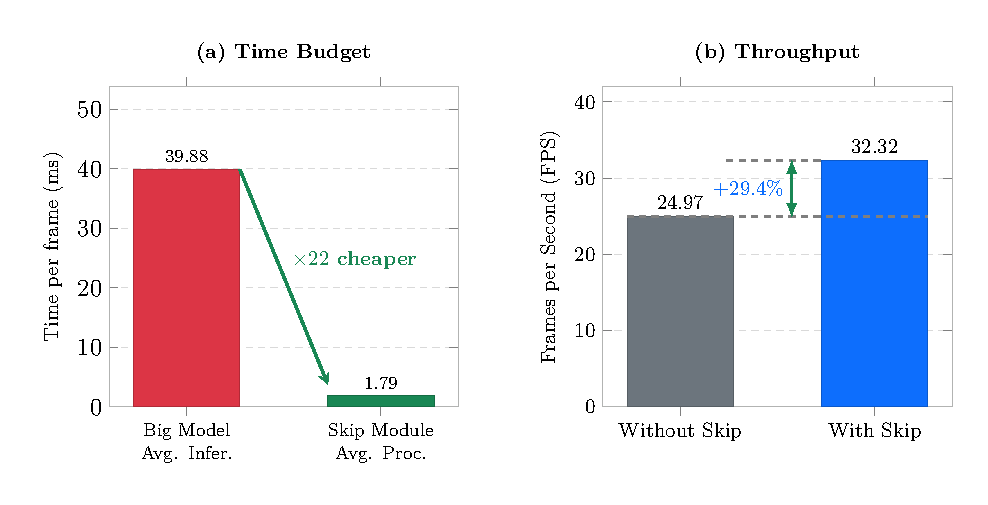
\includegraphics[width=\linewidth,keepaspectratio, scale=0.3]{3.fig/fps_increase.pdf}
  \caption{Proposed pipeline with Skip Frame Mechanism for Indoor Fire and Smoke Detection}\label{fig:fps_increase}
\end{figure}

\section{Conclusion}\label{sec:conclusion}

We propose a lightweight, plug-and-play skip module \(\mathcal{S}\)
designed to accelerate real-time fire and smoke detection in indoor
surveillance scenarios. Operating at a tiny fraction
(\({\approx}2.5\%\)) of the computational cost of the DL classifier
\(\mathcal{M}\), \(\mathcal{S}\) efficiently filters out static
background frames before they reach \(\mathcal{M}\), reducing
unnecessary inference overhead. Experiments on a real-world video
dataset demonstrate that the proposed approach yields a throughput
improvement of over 30\% in frames per second while maintaining
detection reliability.

Nevertheless, the proposed approach has several limitations. First,
\(\mathcal{S}\) relies solely on inter-frame motion cues, which may be
unsuitable for outdoor surveillance scenarios where persistent motion
sources --- such as wind, moving vehicles, etc. --- are continuously
present, potentially causing \(\mathcal{S}\) to pass the majority of
frames to \(\mathcal{M}\) and negating the efficiency gain. Second, the
hyperparameters of \(\mathcal{S}\) require dataset-specific tuning prior
to deployment, incurring additional optimization overhead. Third, the
overall detection accuracy of the system remains bounded by the capacity
of \(\mathcal{M}\), which is treated as a fixed component and not
optimized in this work.

Future work may explore alternative skip strategies --- such as
leveraging color, texture, or learned features as gating cues --- and
extend the framework to outdoor surveillance scenarios where
motion-based filtering is less effective.

\end{document}
